%%%%%%
%
% $Autor: Achal Shakywar $
% $Datum: 2024-08-12 10:40:45Z $
% $Pfad: ML24-EX-Barcode-Reader-with-a-EPS32\Presentations\Achal\Results\slides\content.tex $
% $Version: 2 $
%
% !TeX encoding = utf8
% !TeX root = Rename
%
%%%%%%

	\Mysection{Problem's Description}

\begin{frame}
	\frametitle{Problem's Description}
	
	\begin{block}{}
		Traditional access control systems rely on physical tokens like keys or cards, which can be lost or misused.
		\begin{itemize}
			\item \textbf{Objective}: To develop a secure and contactless face recognition system for simple, private and efficient access control using on-device processing.
			
			\item \textbf{Motivation}: Address the growing demand for efficient authentication by processing data locally on devices, ensuring better privacy and performance.
			
		\end{itemize}
	\end{block}
	
\end{frame}



\Mysection{Description of the Application}
\begin{frame}
	
	
	\frametitle{Description of the Application}
	
	\begin{block}{}
		
		\begin{itemize}
			\item \textbf{DataSet}: Corresponds to three distinct images: Person1, Person2 and Person3.
			\item \textbf{Features}: 
			\begin{itemize}
				\item Facial Feature: Eyes, Nose and Mouth.
				\item Image Type: Grayscale images.
			\end{itemize}
			\item \textbf{Models}:  A CNN-based MobileNetV2 model that can distinguish between different people by learning important features from their facial images, such as facial expressions, to ensure accurate classification.
			\item \textbf{Hardware}: Arduino Portenta H7, Vision Shield and USB-C cable.
			\item \textbf{Software}: Arduino IDE, Edge Impulse CLI, Python, Nodejs and SolidWorks
		\end{itemize}
	\end{block}
	
\end{frame}

\Mysection{Challenges}	
\begin{frame}{Challenges}
	\begin{block}{}
		\begin{itemize}
			\item \textbf{Optimised Image resolution}: Building the model using higher resolutions, such as QVGA (320x240) or lower than QQVGA (128x96) from the Vision Shield camera, led to significant overfitting issues.
			
			\item \textbf{Profile Management}: Attempted to add new profiles and retrain the model in Edge Impulse Studio  using API keys, but faced challenges with API integration.
			
			\item \textbf{Model Accuracy vs. Size}: Keeping the model lightweight for deployment with high accuracy was a challenge.
			
			\item \textbf{Lightning and Environmental Conditions}: Struggled with varying lightning conditions (e.g., too bright or too dark) or environmental factors (e.g., glare or shadows).
			
			\item \textbf{Designing the Mounting and Case}: Struggled to give the 3 DOF to the mounted device.
			
		\end{itemize} 
		
	\end{block}
\end{frame}

\Mysection{Solutions}
\begin{frame}{Solutions}
	
	
	\begin{block}{}
		\begin{itemize}
			\item \textbf{Optimised Image resolution}: Choosing QQVGA (160x120) to balance image quality, reduces overfitting in model building while ensuring accurate recognition.
			
			\item \textbf{Profile Management}: Preferred manually update the dataset and retrain the model in Edge Impulse Studio \cite{edgeimpulse:2025}, prioritizing accuracy over automation.
			
			\item \textbf{Model Accuracy vs. Size}: Used model Quantization(int8) \cite{mathworksint8quantization:2025} techniques to reduce the model size without sacrificing accuracy.
			
			\item \textbf{Lighting and Environmental Conditions}: Ensure optimal hardware placement in environments with balanced lighting to reduce the impact of glare, shadows, and extreme brightness.
			
			\item \textbf{Designing the Mounting and Case}: Designed the prototype on solidworks.
			
		\end{itemize}
		
	\end{block}	
\end{frame}		

\begin{frame}
	\begin{figure}[h!]
		\centering
		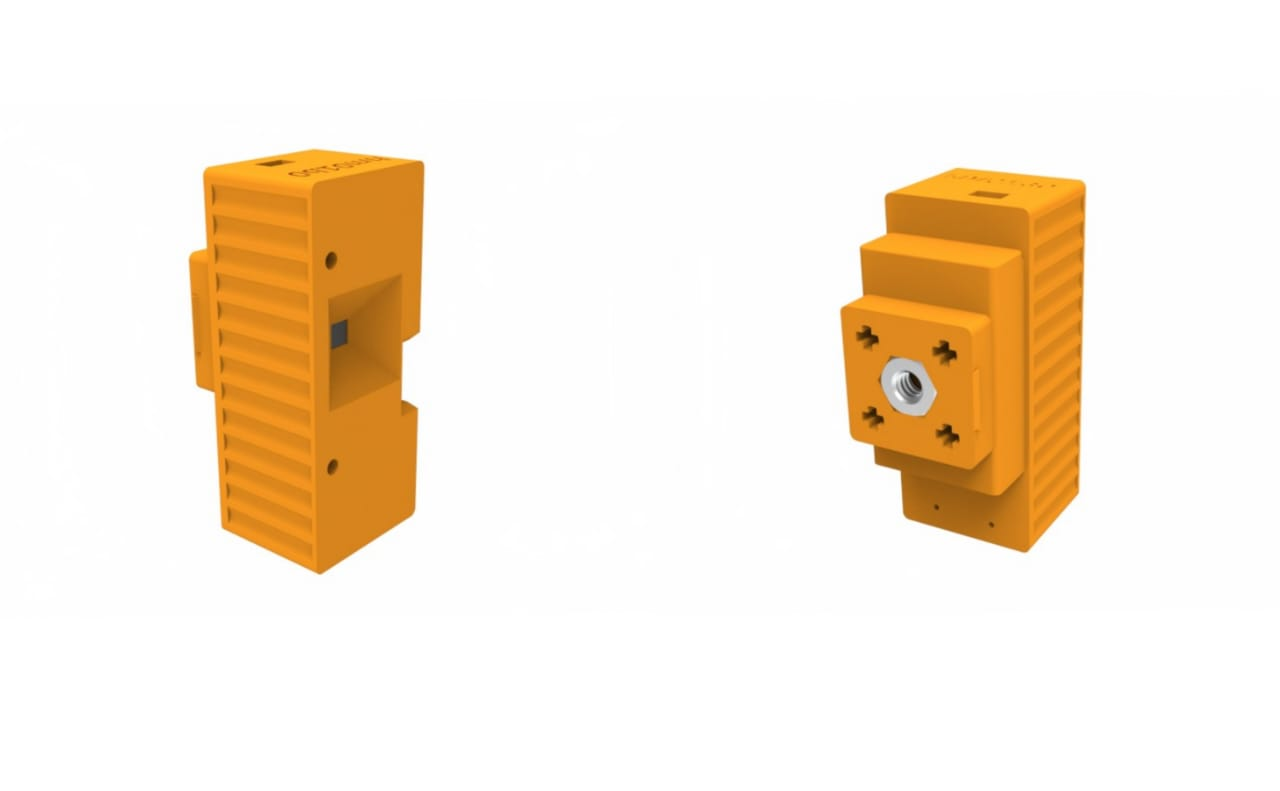
\includegraphics[width=0.9\textwidth]{images/PoretentaVisionShieldCover.jpg}
		\caption{Portenta Vision Shield Cover}
		\label{Cover}
	\end{figure}
\end{frame}


\Mysection{Results}
\begin{frame}[allowframebreaks]{Results}
	\begin{block}{Configuring Training Parameters}
		\begin{itemize}
			
			\item The optimized model achieved accuracy of \textbf{85.2\%} during testing, effectively recognized  faces across all trained profile.
			
			\item Achieved \textbf{1789ms}  inference time per frame, enabled smooth recognition on Portenta H7. 
			
			\item Successfully handled varied light conditions with the balanced dataset.
			
			\item The system supported profile updates and deletions, ensuring flexible and efficient access control. 
			
			
		\end{itemize}
	\end{block}

\begin{table}[h!]
	\centering
	\small % Reduce the font size of the table
	\caption{Validation Result}
	\begin{tabular}{|p{3cm}|p{3cm}|} % Set fixed column widths
		\hline
		\textbf{Validation Set}             & \textbf{Values}                                  \\ \hline
		Accuracy                    &  85.2\%       \\ \hline
		Loss               & 0.41 \\ \hline
		Average Precision                     & 0.90 \\ \hline
		Average Recall                  & 0.85   \\ \hline
		Average F1 Score           & 0.84 \\ \hline

	\end{tabular}
	\label{tab: Validation_Result}
\end{table}

\begin{table}[h!]
	\centering
	\small % Reduce the font size of the table
	\caption{Performance Metrics}
	\begin{tabular}{|p{3cm}|p{3cm}|} % Set fixed column widths
		\hline
		\textbf{Performance Metrics}             & \textbf{Values}                                  \\ \hline
		Inferencing Time                    &  1789ms       \\ \hline
		Peak Ram Usage              & 280.9k \\ \hline
		Flash Usage                    & 358.2k \\ \hline
		
	\end{tabular}
	\label{tab: Performance_Metrics}
\end{table}


	
\begin{figure}[h!]
	\centering
	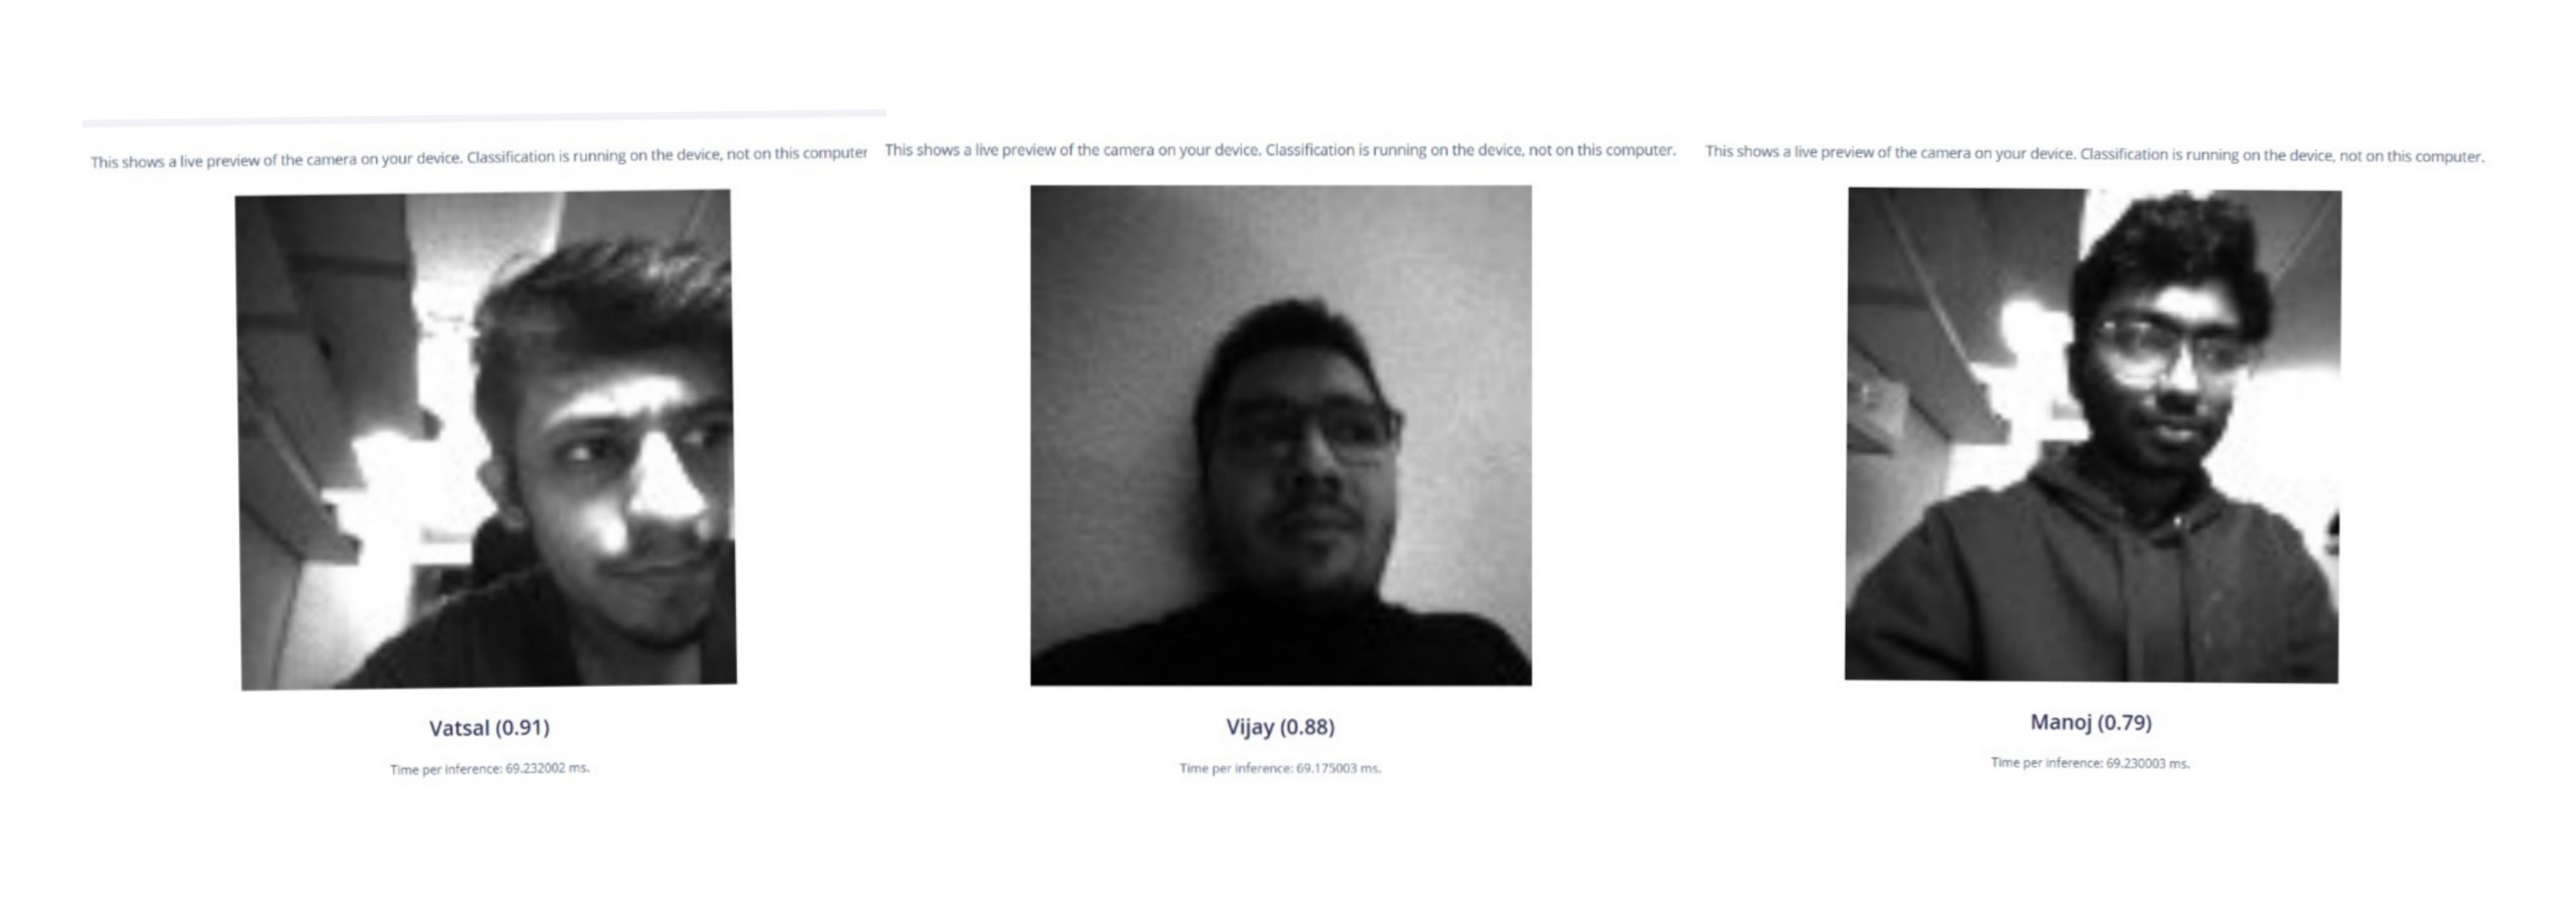
\includegraphics[width=0.9\textwidth]{images/Result.jpg}
	\caption{Output of the Face Recognition System}
	\label{fig:Output}
\end{figure}




\end{frame}

